\newpage
\section{Contiki measurements distribution}

By comparing the measures made with Contiki to the one made with RIOt, we notice a huge difference.
With RIOT, the standard deviation is 31.16ns with the RE-Mote board and 27.61ns with the Z1 board.
With Contiki, the standard deviation is $10\mu s$ with the RE-Mote board and $54\mu s$ with the Z1 board.
The figure \ref{fig:deviation-ref-value-remote} and the figure \ref{fig:deviation-ref-value-z1} clearly show the difference between the distribution of the reference value between Contiki and RIOT.
At this point, we do not know where this difference comes from.

\begin{figure}[!ht]
  \centering
  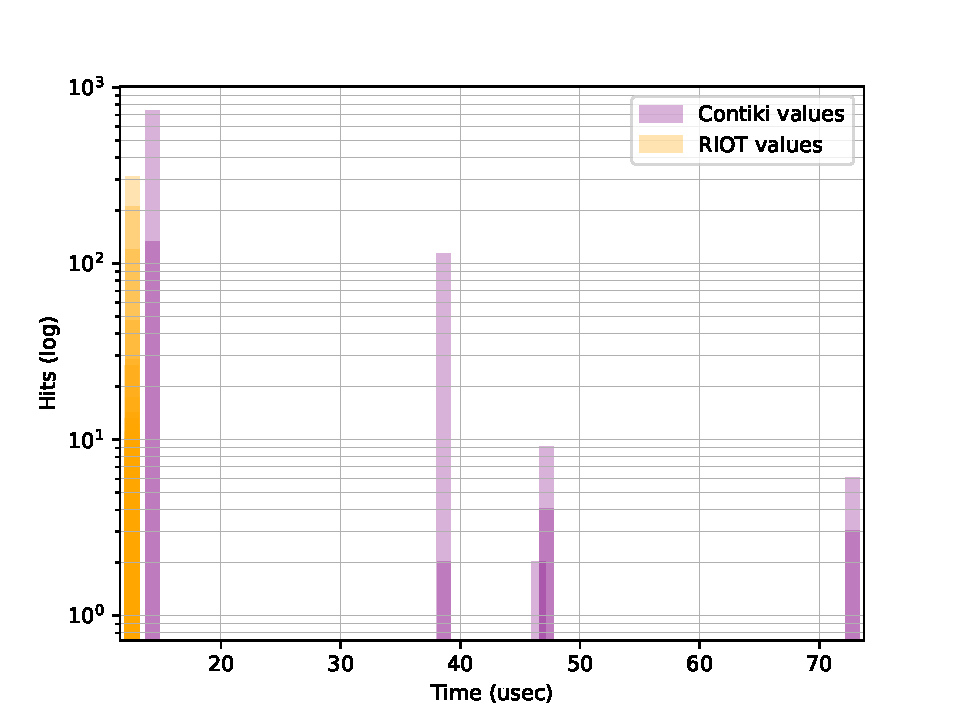
\includegraphics[scale=.7]{assets/offset-remote.pdf}
  \caption{distribution comparison between RIOT and Contiki with the reference value on the RE-Mote board\label{fig:deviation-ref-value-remote}}
\end{figure}

\begin{figure}[!ht]
  \centering
  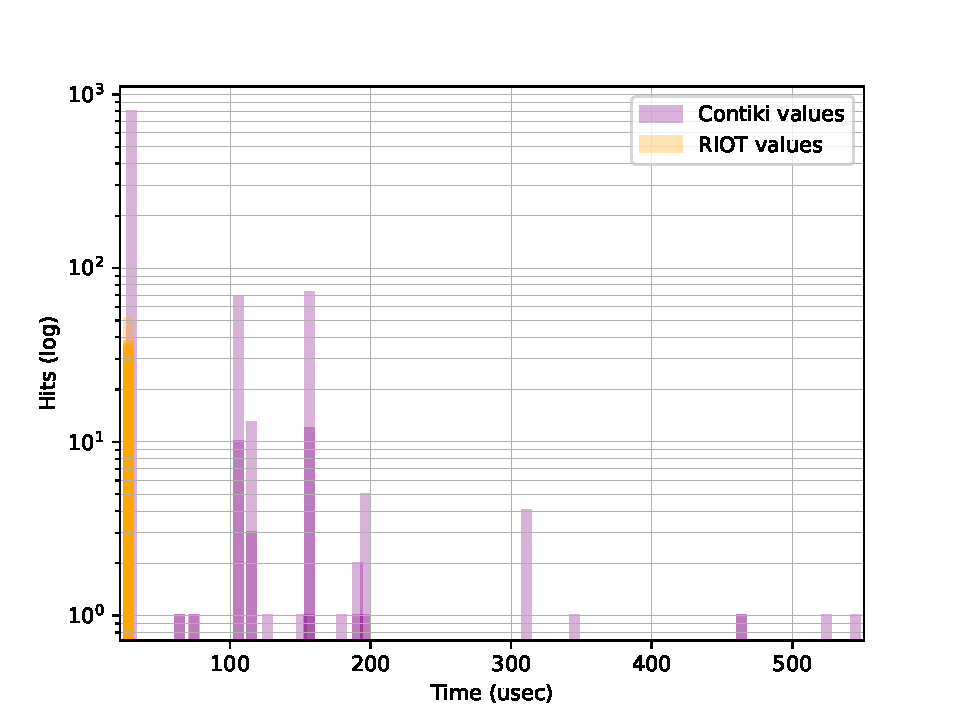
\includegraphics[scale=.7]{assets/offset-z1.pdf}
  \caption{distribution comparison between RIOT and Contiki with the reference value on the Z1 board\label{fig:deviation-ref-value-z1}}
\end{figure}